\documentclass{beamer}

% Theme choice (you can change to Madrid, CambridgeUS, etc.)
\usetheme{Madrid}

% Optional packages
\usepackage[utf8]{inputenc}
\usepackage{graphicx} % for including images
\usepackage{amsmath, amssymb, mathtools} % for math symbols
\usepackage{hyperref} % for clickable links
\usepackage{tikz}

% Title info
\title[Short Title]{Systematic Trading from First Principles}
\author[Your Name]{Oden Petersen}
\date{\today}

% Section headers
\AtBeginSection[]{
	\begin{frame}
	\vfill
	\centering
	\begin{beamercolorbox}[sep=8pt,center,shadow=True,rounded=True]{title}
		\usebeamerfont{title}\insertsectionhead\par%
	\end{beamercolorbox}
	\vfill
	\end{frame}
}

\begin{document}

% Title page
\begin{frame}
	\titlepage
	\begin{center}
		\textit{``$y=X\beta+\epsilon$, the rest is commentary.''}
	\end{center}
\end{frame}

\begin{frame}{About Me}
\end{frame}

\begin{frame}{Point of This Talk}
	%mathematical language. why
		%lotta moving parts. ambiguities can add up
		%ill give the economic intuition behind things anyway
	%increasingly lowfreq and highfreq trading styles are converging. common basis needed
	%axiomatic like euclid
	%not talking how to get job. in efficient market the way to get job is just to be good at the work
	%Not directly talking about how to do the job either
		%The kind of rigour here is about precise communication of the concepts.
			%Communication at work focuses much more on concrete facts, relies on greater implicit shared context.
			%Many of the best traders would have no idea what you mean if you just speak in maths
		%The work itself is often extremely heuristic by necessity. The ability to appreciate which parts of the problem are most important represent things in a simple way while capturing the important qualitative parts is a key skill in both manual and systematic trading
\end{frame}
% Table of contents
\begin{frame}{Outline}
	\tableofcontents
	%% Good to include concrete data examples throughout
	%% Make sure := for definitions
\end{frame}

\section{Securities Markets}

\begin{frame}{Spot Transactions}
	The point of trading is to obtain an asset by giving up money, or obtain money by giving up an asset.%Counterexample: currency triangles

	If I give $q>0$ units of some asset $A$, and you give me $\$p$, then:%I'm gonna use dollar signs here although often we trade in many currencies. It is typical to emphasise one currency which we call the numeraire and express things in terms of it.
	\begin{itemize}
		\item I have \textbf{sold} $q$ units of $A$ to you at $\frac{\$p}{q}$
		\item You have \textbf{bought} $q$ units of $A$ from me for $\frac{\$p}{q}$
	\end{itemize} %"for" and "at" indicate direction

	Buying and selling are collectively called `trading'.%One trade can have multiple counterparties, we will see this later

	Suppose I own some amount of $A$ and some amount of money. If we let $s$ be $+1$ for buying and $-1$ for selling, then the result of any trade is to add $qs$ to the amount of $A$ I own, and add $-qps$ to the amount of money I have. %s is called the sign of the trade

	% Stock image of retail store
\end{frame}

\begin{frame}{Securities Markets and Exchanges}
	The \textbf{\textcolor{blue}{market}} is the collective activity of all traders. When we don't care who we trade with, we can just `trade with the market'.

	A \textbf{\textcolor{red}{securities} \textcolor{blue}{market}} for some asset $A$, open at a time $t$, is any \textcolor{red}{standardised} \textcolor{blue}{way for traders to reach agreements to buy or sell} $A$ at a specified \textbf{settlement time} $T\geq t$. %"securities" because of standardisation and regulation. Agreements are often treated as the same as trades, though there are some cases where the distinction matters

	\pause

	For example, $T=\ldots$
	\begin{itemize}
		\item $t$ (`spot', e.g. blockchain) %ASX tried to do blockchain, this was scrapped in 2022 after 7yrs
		\item $t+1, t+2, \ldots$ (`clearing', e.g. equities)
		\item Last Thursday of month (`futures')
	\end{itemize}

	\pause
	If you agree to give something to someone, you have an \textbf{obligation}. If someone agrees to give you something, you have a \textbf{right}.

	\begin{block}{Counterparty Risk}
		If I have an agreement with $P_1$ to buy $10$ units for $\$p_1$ at $T$, and an agreement with $P_2$ to sell $10$ units at $\$p_2$ at $T$, and no further rights/obligations, am I guaranteed to meet my obligations?
	\end{block}%Define counterparty risk
\end{frame}

\begin{frame}{Centralisation}
	A \textbf{securities exchange} is a centralised venue serving a securities market for \textbf{exchange participants} (e.g. ASX, NYSE, TSE, HKEX, LME).

	Agreements not made through an exchange are often called OTC (over-the-counter). %Also called off-exchange. Define search costs.

	\begin{center}
		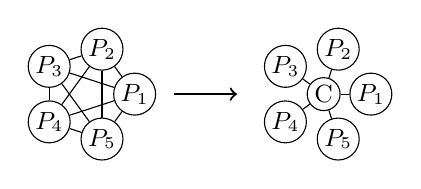
\begin{tikzpicture}[baseline, every node/.style={circle, draw, fill=white, inner sep=1pt, font=\small, minimum size=1mm}]
			\foreach \i in {1,...,5} {
				\node (n\i) at ({72*(\i-1)}:0.6) {$P_{\i}$};
			}
			\foreach \i in {1,...,5} {
				\foreach \j in {1,...,5} {
					\ifnum\i<\j
						\draw (n\i) -- (n\j);
					\fi
				}
			}

			\draw[->, thick] (1.1,0) -- (1.9,0);

			\begin{scope}[xshift=3cm]
				\node (c) at (0,0) {C};
				\foreach \i in {1,...,5} {
					\node (n\i) at ({72*(\i-1)}:0.6) {$P_{\i}$};
					\draw (c) -- (n\i);
				}
			\end{scope}
		\end{tikzpicture}
	\end{center}

	Centralisation generally reduces \textbf{search costs} and \textbf{counterparty risk}. %Mention risk counterexample: FTX vs a DEX
\end{frame}

\begin{frame}{Netting}
	Centralisation allows for \textbf{netting} of rights and obligations.

	For any settlement time $T$, I only need to keep track of the difference between money owed to and by me, and units owed to and by me.

	The quantity of $A$ owned by me, plus the quantity owed to me, minus the quantity owed by me to others, is known as my \textbf{net position} in $A$.

	If this is positive, I have a \textbf{long position}. If it is negative, I have a \textbf{short position}. If it is zero, I am \textbf{flat}.
\end{frame}

\begin{frame}{Collateralisation}
	At certain intermediate times $t'$ ($t\leq t'\leq T$), participants may be required to physically give (`post') something to the exchange to \textbf{collateralise} their obligations.
	\begin{itemize}
		\item Money (`margin') %Explain the term "futures type settlement" and "stock type settlement"
		\item Assets (`locate'/`borrow') %"Borrow" is only if you don't own the thing
	\end{itemize}
	If an agreement made on the exchange gives you rights to money or assets at $T$, this is typically as good as posting actual money or assets for an obligation at $T'\geq T$.
	%Interest rates, borrow rates etc
\end{frame}

\begin{frame}{Summary}
	\begin{itemize}
		\item \textbf{Trading} is swapping money and assets
		\item A \textbf{market} is whatever you use to trade
		\item A \textbf{securities market} is a standardised way to agree to trades
		\item Agreements consist of \textbf{rights} and \textbf{obligations}
		\item Finding a \textbf{counterparty} may involve \textbf{search cost}
		\item Agreements between two parties are subject to \textbf{counterparty risk}
		\item A \textbf{securities exchange} is a centralised trading venue %Maybe explain national market system
		\item After trades are agreed to on an exchange, they will be \textbf{settled} in some standardised way
		\item The net quantity of $A$ that I have some claim to can either be positive (\textbf{long position}), negative (\textbf{short position}), or zero (\textbf{flat}).
		\item Traders may be obligated to post assets ('locate') or money ('margin')
	\end{itemize}
\end{frame}

\section{Trading}
\begin{frame}{Setup}
	A sequence of trades that collectively increases the amount of money you have and leaves the amount of each asset you have unchanged is clearly favourable.

	\pause

	Suppose that at each time $t$ we have cash holdings of $\$c_t$ and net holdings of $a_t$ units of some asset $A$.

	Suppose also that trades $(s_t, q_t, \$p_t)$ take place at a finite set of distinct times
	$$\tau = \{t_1,\ldots t_n\}\subset T = [t_-, t_+],$$
	where $t_-<t_1<\ldots<t_n<t_+$.

	\pause

	Suppose further that $p_t$ is a right-continuous function $\mathbb R\to\mathbb R$ with left-limits.

	For instance, we could take $p_t = p_{\max \left(\tau\cap (-\infty,t]\right)}$ for $t\geq \min\tau$ and $p_t=x$ otherwise for some arbitrary $x$. This is known as the last traded price.
\end{frame}

\begin{frame}{Accounting}
	For any time-varying quantity $x_t$, let $x_t^+$ and $x_t^-$ denote the right- and left-limits respectively.

	Furthermore, define a signed measure $x_\omega$ such that for any interval $T'=[t_-',t_+']$ we have
	$$x_{T'} := x_{t_+}^+ - x_{t_-}^-.$$

	\pause

	Then we have

	\vspace{-0.06\textheight}
	\begin{align*}
		a_{T'}	&= \sum_{t\in \tau} s_t q_t		&&= \int_{t\in T} da,
	\\	c_{T'}	&= \sum_{t\in \tau} - p_t (s_t q_t)	&&= \int_{t\in T} - p_t da,
	\\	p_{T'}	&= p_{t_+'} - p_{t_-'}^-.		&&= \int_{t\in T} dp.
	\end{align*}%Special case: t_-'=t_+'
\end{frame}

\begin{frame}{Cash Holdings}
	It can be shown (see appendix) that the cashflow over the entire interval $T=[t_-,t_+]$ is
	$$\$c_T = \int_{t\in T} - \$p_t da = \$p_{t_-}a_{t_-} - \$p_{t_+}a_{t_+} + \$\int_{t\in T} a_t^- dp.$$
	This is similar in spirit to integration by parts:
	$$\int_a^b f \frac{dg}{dx} dx = f(b)g(b)-f(a)g(a) - \int_a^b g \frac{df}{dx} dx.$$

	Then we have
	$$\$(c_{t_+} + p_{t_+}a_{t_+}) - (c_{t_-} + p_{t_-}a_{t_-}) = \$\int_{t\in T} a_t^- dp.$$

	The quantity $\$v_t = \$p_t a_t$ is known as the \textbf{dollar value} of our $A$ holdings \textbf{marked} to the price $\$p_t$.%Marking just means multiplication of units held by a unit price
\end{frame}

\begin{frame}{Portfolio Valuation}
	Suppose now that we trade multiple assets, such that $p_t$, $a_t$ and $v_t$ are vector-valued, with $v_t$ the elementwise product of $p_t$ and $a_t$.

	A collection of assets held in quantities $a_t$ is known as a \textbf{portfolio}.

	\pause

	We can write
	$$(c_{t_+} + p_{t_+} \cdot a_{t_+}) - (c_{t_-} + p_{t_-} \cdot a_{t_-}) = \int_{t\in T} a_t^- \cdot dp,$$
	where $p_\omega$ is now a vector-valued measure. \pause Let
	$$\Pi_t	= c_t + p_t\cdot a_t = c_t + \sum v_t.$$

	We call $\$\Pi_t$ the \textbf{value} of our portfolio \textbf{marked} to $p_t$.
\end{frame}

\begin{frame}{Profitability}
	The quantity $\$\Pi_{t_+} - \$\Pi_{t_-}$ is our \textbf{net P\&L} (profit and loss) over the interval $T$, marked to $p_t$.
	Then we have
	$$\Pi_T	= \int_{t\in T} a_t^- \cdot dp.$$
	we can write
	$$\Pi_{[t_i,t_{i+1}]} = \int_{[t_i,t_{i+1}]} a_t^- \cdot dp = \int_{t\in [t_i, t_{i+1}]} v_t^- \cdot \frac{dp}{p_t^-},$$
	where the quotient $\frac{dp}{p_t^-}$ is computed elementwise.
\end{frame}

\begin{frame}{Leverage}
	Suppose we can always make any trade we like at time $t$ with price $\$p_t$. %Not a terrible guess if we did indeed make some trade at $\$p_{t_i}$.

	Then we can freely convert a portfolio with value $\$\Pi_t$ to that much in cash.

	Conversely, we can convert $\$\Pi_t$ worth of cash into any portfolio with that value.

	In practice, there are limits on the trades we can make at a particular price and time.

	\pause

	Typically, $\$\Pi_t$ can change in two ways: trading assets, or transferring cash into and out of the portfolio. We will generally ignore the possibility of transfers.

	\pause

	If we begin with a portfolio worth $\$\Pi_{t_1}$ and make a sequence of trades of the form $(s_t,q_t,p_t)$ that result in a portfolio worth $\$\Pi_{t_n}$, then we could instead begin with a portfolio worth $L \$\Pi_{t_1}$ and make trades $(s_t, L q_t, p_t)$ to arrive at a portfolio worth $L \$\Pi_{t_n}$. The ratio $L$ is known as the \textbf{leverage ratio}.
\end{frame}

\begin{frame}{Return on Capital}
	Because of collateralisation requirements, portfolio management uses up cash.

	Consider long-only spot-settled trading. If we were to turn our portfolio into cash, or convert cash into an identical portfolio, we would receive/require $\$\Pi_t$.\footnote{We generally want $c_t$ to be small, but we may want some spare cash for trading, so it still forms part of the collateralisation requirement.}%For a long-short portfolio with no borrow costs, the collateral requirement is generally at least $c_t + \vert a_t\vert \cdot c_t$. The calculations are different for margined trading eg futures. Complexity i wont go into. Maybe appendix?

	%To judge trading efficiency, we might want an estimate for how much extra P\&L over the interval $T$ would result from a marginal dollar added to $\$\Pi_t$.
	\pause

	If our initial portfolio value were $\$\Pi_{t_-}+\$N$ instead of $\Pi_{t_-}$, and we could simply scale up trade sizes at the same prices, then set
	$$L = \frac{\Pi_{t_-}+N}{\Pi_{t_-}}.$$

	\pause

	The \textbf{return on capital} is defined as the increase in P\&L per dollar added to initial portfolio value, i.e.
	$$R_T = \frac{L \int_T d\Pi - \int_T d\Pi}{N} = \frac{\int_T d\Pi}{\Pi_{t_-}}.$$
\end{frame}

\begin{frame}{Log Returns}
	If we define
	$$\ell_t = \log \Pi_t$$ %sometimes called log-wealth
	for any $t_-',t_+'$, then we have
	$$R_T = \exp(\ell{l}_T) - 1,$$
	and for any measurable set $\omega$ we can define
	$$R_\omega = \exp(\ell_\omega) - 1 \approx \ell_\omega + O(\ell_\omega^2)\textrm{ (for small }\ell_\omega\textrm{)}.$$

	We call $\ell_T$ the \textbf{log-return} over the interval $T$.
\end{frame}

\begin{frame}{Properties of Returns and Log-Returns}
	Let $w_t := \frac{1}{\Pi_t}v_t$ be the \textbf{weight vector}.%Explain interpretation

	For an interval $T' = (t_i,t_{i+1}]$, we have $a_t^-$ equal to a constant over $T'$, and
	$$R_{T'} = w_{t_i}^+ \cdot r_{T'},$$
	where the elementwise quotient
	$$r_{T'} = \frac{p_{t_{i+1}} - p_{t_i}}{p_{t_i}}$$
	is known as the \textbf{asset returns} vector over $T'$. In contrast, $\ell_{T'}$ is not linear in $r_{T'}$. %In fact there's no function of the return that \ell_{T'} is linear in. Benefits and drawbacks, eg expectation/variance

	For a disjoint collection of measurable sets $\omega_1,\ldots\omega_n$ whose union is $\Omega$, we have
	$$\ell_\Omega & &= \sum_{i=1}^n \ell_{\omega_i},$$
	$$R_\Omega &= \left(\prod_{i=1}^n (1+R_{\omega_i})\right) - 1 &\approx \sum_{i=1}^n R_{\omega_i} + O\left(\sum_{i=1}^n\sum_{j=1}^n \vert R_{\omega_i} R_{\omega_j} \vert\right).$$
\end{frame}

\begin{frame}{Summary}
	\begin{itemize}
		\item 
	\end{itemize}
\end{frame}

\section{Market Microstructure}
\begin{frame}{Trade Formation}
	In practice, the trades we can make at a time $t$ and a price $p_t$ are limited by our ability to find a willing counterparty.

	\pause
	On an electronic exchange, trades are formed by interacting with the exchange's \textbf{matching engine}.%Matching engine is a computer networked with the computers of exchange participants. Usually the algorithm is mostly deterministic and publicly known, but this is not always the case and knowledge of the matching engine can give you an advantage over other traders

	\pause

	For each trade $(s,q,\$p)$, the exchange will typically charge a fee proportional to the \textbf{dollar volume} $\$pq$ of the trade. Fee rates may vary depending on trade type and between participants in accordance with exchange policy.

	\pause

	The most common type of matching engine design is a \textbf{limit-order book} (sometimes called a double auction), which can operate in either a \textbf{continuous} or \textbf{batched} fashion.
\end{frame}

\begin{frame}{Limit Order Book}%Special kind of data structure
	At any point in time, market participants can create a request (`\textbf{limit order}') of the form $(s,q,\$p)$ to trade up to $q$ units in direction $s=\pm1$ at any price $\$(p-sm), m\geq0$.%If I'm happy to buy for at most 10 then I'm happy to buy for 1 since this would be a price improvement of 9

	The value $\$m$ is known as the \textbf{price improvement}. %The request poster prefers large m. $p is sometimes called the reserve price
	
	They are then said to be ``\textbf{bid} for $\$p$'' ($s=+1$) or ``\textbf{ask}ing/\textbf{offer}ing at $\$p$'' ($s=-1$). %Bid and ask are terms referring to limit order directionality. for and at also indicate direction, as mentioned before

	\pause

	All limit orders active at time $t$ are collected into a \textbf{limit-order book} $\mathcal{L}_t$. By convention, $\mathcal{L}_t$ is right-continuous with left limits.%multiset

	Users can add, cancel and modify orders, subject to exchange-specific rules.%Limits on modification. Ratelimits, message limits etc. GFD etc - FOK FAK explained later
\end{frame}

\begin{frame}{Order Matching}
	Whenever $(+1,q_1,\$p_1), (-1,q_2,\$p_2)\in\mathcal{L}_t$ with $p_2\leq p_1$, both orders could be at least partly satisfied by trading up to $q_{\max}=\min(q_1,q_2)$ units with one another at a price $\$p\in[\$p_2,\$p_1]$. If such a pair exists the book is said to be \textbf{in cross}.

	\pause

	If an order $(s,q,\$p)$ is in cross with another, it may be \textbf{matched} for $q'$ units. The total matched quantity for all buy orders must equal the total matched quantity for all sell orders.

	\pause

	In this case, $q'$ units will trade, and the order will become $(s,q-q',\$p)$.

	\pause

	If $q=q'$ the order is said to be \textbf{fully filled} and will be removed from the book. Otherwise, it is said to be \textbf{partially filled}.

	\pause
	The ability to quickly find matches for a large number of units at a reasonable price is known as \textbf{liquidity}, and is another major benefit of centralisation.
\end{frame}

\begin{frame}{Supply and Demand Curves}
	We can partition $\mathcal{L}_t$ into $\mathcal{L}_t = \mathcal{B}_t\cup\mathcal{A}_t$, with $\mathcal{B}_t$ the bid orders and $\mathcal{A}_t$ the ask orders.

	\pause

	Now define the functions
	\begin{align*}
		Q_t(+1,\$p)	&= \sum_{\substack{(+1,q',\$p') \in \mathcal{B}_t \\ \$p\leq \$p'}} q'
	\\	Q_t(-1,\$p)	&= \sum_{\substack{(-1,q',\$p') \in \mathcal{A}_t \\ \$p\geq \$p'}} q'
	\\	M_t(\$p)	&= \min(Q_t(+1,\$p),Q_t(-1,\$p))
	\end{align*}
	\pause
	The functions $Q_t(-1,\$p)$ and $Q_t(+1,\$p)$ are known as the \textbf{supply curve} and \textbf{demand curve} respectively. The function $M_t(\$p)$ represents the \textbf{matchable quantity} at $\$p$.
	\pause
	The book $\mathcal{L}_t$ is in cross if and only if there exists some $\$p$ with $M_t(\$p)>0$.
	%Diagram. separate slide
\end{frame}

\begin{frame}{Batch Matching}
	In \textbf{batch} or \textbf{auction} style matching, orders are matched with one another only at particular discrete times.

	\pause

	\begin{enumerate}
		\item Prior to the \textbf{match time} $t^*$, users can typically add, modify and cancel limit orders.
		\item At each time $t\leq t^*$, an \textbf{indicative price} $\$p^*_t$ will be selected such that $M_t(\$p^*_t)$ is maximal. Tiebreaking will depend on exchange rules.
		\item Finally, at the match time $t^*$, some subset of the crossed limit orders will be matched at $\$p^*$ for a total quantity $M_{t^*}(\$p^*_{t^*})$. After the match, the book will no longer be crossed.
	\end{enumerate}

	\pause

	Maximising $M_t(\$p^*_t)$ is equivalent to maximising the sum of $qm$ across all orders, where $q$ is the quantity filled and $m$ is the price improvement.%Also maximises fees paid

	It is common to use this matching style at the beginning or end of a trading day or lunch break, or when there is some kind of market instability such as following a large price move or company announcement. Sometimes $t^*$ is referred to as a \textbf{liquidity event} because of the large volume traded, and the relative insensitivity of $\$p^*_{t^*}$ to individual orders.%Price impact nonnegative because of monotonicity property
\end{frame}

\begin{frame}{Batch Matching Properties}
	The following monotonicity properties typically hold:
	\begin{itemize}
		\item $\$p^*_t$ nondecreasing in $\mathcal{B}_t$ and nonincreasing in $\mathcal{A}_t$
		\item For each $\$p$, $M_t(\$p)$ nondecreasing in $\mathcal{L}_t$
		\item For individual orders $(s,q,\$p)$, we will have $\$p^*_t$ nondecreasing in $\$p$ and $sq$. %The sensitivity of the match price to the parameters of the individual order is known as the instantaneous price impact.
		\item For individual orders $(s,q,\$p)$ and each $\$p'$, we will have $M_t(\$p')$ nondecreasing in $q$ and nondecreasing in $\$sp$.
	\end{itemize}

	\pause

	\begin{block}{Price Priority}
		Because $M_t(\$p')$ is nondecreasing in $sp$, the matching will be designed to obey \textbf{price priority}.
	
		If we have two orders $(s_1,q_1,\$p_1), (s_2,q_2,\$p_2)$ with $\$s_1p_1 > \$s_2p_2$, then the second order cannot be matched unless the first is completely filled.
	\end{block}
\end{frame}

\begin{frame}{Order Timing}
	The order book is often visible to all participants. Traders may be incentivised to wait until immediately before the match time to post orders.%Hiding intentions, using all information available

	\pause

	If everyone does this, the matching engine may be overloaded, and $p^*_t$ will change very rapidly leading up to $t^*$.

	\pause

	The match time is typically chosen at random in some short interval in order to disincentivise this behaviour.
	\pause
	To further encourage early submission of orders, many exchanges also implement a time priority rule.%As opposed to pro rata
	\begin{block}{Time Priority}
		If two orders exist at the same price $\$p$, the one that reached the matching engine later cannot be matched unless the earlier order is completely filled.
	\end{block}

	\pause

	\begin{block}{Tick Size}
		Time priority would not have much effect if we could just insert the later order at a price $\$p+s\epsilon$ for some very small $\epsilon>0$.%Because of price priority. "Diming"

		To avoid this, prices must be integer multiples of some small increment $\$\delta$, known as the \textbf{tick size}.%Sub-penny rule reg nms
	\end{block}
\end{frame}

\begin{frame}{Continuous Matching}
	In \textbf{continuous matching}, a match time is triggered every time a new limit order causes the book to become crossed.

	\pause

	If the matching engine receives an order at $t$, then immediately before and after $t$ the book will be uncrossed, with $M_t(\$p)=0$ at all $\$p$.

	\pause

	The only orders involved in the match will be the arriving order and some set of orders $\mathcal{M}_t$ in the opposite direction.

	The arriving order is known as the \textbf{active} or \textbf{aggressive} order, and the pre-existing orders are known as \textbf{passive}.%Also known as taker and maker orders. Sometimes have different fees

	Typically we are not allowed to match with ourselves. Often the exchange will implement \textbf{self-trade protection} so that the quantity of our active and passive orders is simply cancelled out without recording a trade.

	Price priority is still used, and time priority is usually used.

	% Passive orders provide liquidity to anybody who wants to trade. This liquidity goes away when traded against, so latency matters. Adverse selection comes into play here

	\pause

	For each $q'$ matched against a passive order $(s,q,\$p)$, the active order will trade $q'$ units with the passive order at $\$p$. %Unlike auction-style matching, there may be multiple trade prices according to the prices of the passive orders. No price improvement for passive orders

	\pause

	The per-unit price achieved by the active trader will be
	$$\$p^*_t = \frac{\sum_{(s,q,\$p)\in\mathcal{M}_t} \$pq}{\sum_{(s,q,\$p)\in\mathcal{M}_t} q}.$$ %This may or may not be a multiple of the tick size.

	%Market orders
	%Usually used for intraday trading

	% order priority -> latency -> colocation, fpgas.
	%adverse selection -> order priority. + free messages -> tick size, min size, lot size, ratelimits.
	% "Certainly, the modern compendium of mental illnesses (DSM-5) takes a dim view of people who think everyone is out to get them. Yet financial markets are different: people really are out to get you, after all." - Agustin Lebron, The Laws of Trading

	%FAK,FOK
\end{frame}

\begin{frame}{Instantaneous Price Impact}
	If we aggressively trade a very large quantity, we will exhaust all passive orders we would most prefer to trade with and $\mathcal{M}_t$ will need to include orders at worse price levels. This is sometimes known as \textbf{walking the book}.

	\pause

	Assume continuous matching, and consider a market order of $q>0$ units in direction $s$.

	\pause
	The least favourable price in $\mathcal{M}_t$ will be given by
	$$\$P_t(sq) = s\min_{\{\$p : Q_t(-s,p)\geq q\}} \$sp.$$

	\pause

	The unit price of the match will be given by
	$$\$p^*_t(sq) = \frac{1}{q}\int_0^q \$P_t(sq')dq'.$$

	We call the sensitivity of $\$p^*_t$ to $sq$ the \textbf{instantaneous price impact}.%Sometimes known as transient price impact
\end{frame}

\begin{frame}{Bid-Ask Spread}
	We call the prices
	\begin{align*}
		\$b_t	&= \lim_{q\to0^+} \$p^*_t(-q)	&&= \max_{(+1,q,\$p)\in\mathcal{B}_t} \$p
	\\	\$a_t	&= \lim_{q\to0^+} \$p^*_t(q)	&&= \min_{(-1,q,\$p)\in\mathcal{A}_t} \$p
	\end{align*}
	the \textbf{bid price} and \textbf{ask price} respectively. All bid orders have price at most $\$b_t$ and all ask orders have price at least $\$a_t$.%To trade an infinitesimal amount, we would need to sell at $\$b_t$ or buy at $\$a_t$.

	The interval $[\$b_t,\$a_t]$ is known as the \textbf{spread}, and $\$a_t-\$b_t$ is the \textbf{width} of the spread. If $\$a_t-\$b_t=\$\delta$, we say that the market for the asset is \textbf{large-tick} or \textbf{tick-constrained}.%Proxy for liquidity

	%Cross-listing arbitrage (incl. fees) when spreads are disjoint (union of L_t and L_t' is 'in cross'). We can perform the matching ourselves and possibly make money net of fees
		%PFOF
		%Collateralisation considerations - often not netted
		%Latency risk
\end{frame}

\begin{frame}{Price Proxies}
	Note that $\$p^*_t(0)$ is not yet defined. So long as we choose some price $\$m_t$ satisfying $\$m_t\in[\$b_t,\$a_t]$, setting $\$p^*_t(0) := \$m_t$ will make $\$p^*_t(\cdot)$ nondecreasing.

	\pause

	This is variously called the \textbf{theo}retical price, \textbf{microprice} or \textbf{price proxy} depending on context.

	\pause

	Some simple choices for $m_t$ include:
	\begin{itemize}
		\item $\frac{1}{2}b_t+\$\frac{1}{2}a_t$ (arithmetic \textbf{midprice})
		\item $\$\sqrt{b_ta_t}$ (\textbf{geometric midprice})
		\item $\$(1-I_t)b_t + \$I_ta_t$ (depth-$\$d$ \textbf{weighted midprice})
		\item $\$b_t^{1-I_t}a_t^{I_t}$ (depth-$\$d$ \textbf{geometrically weighted midprice})
	\end{itemize}
	We call $I_t$ the \textbf{book imbalance}.

	\pause

	A popular choice for this is
	$$I_t=\frac{Q_t(+1,\$b_t)}{Q_t(+1,\$b_t)+Q_t(-1,\$a_t)}.$$

	Alternative price proxies are described in the appendix.
	% Microstructural noise -> Roll model
\end{frame}

\begin{frame}{Persistent Price Impact}
	We call the difference $\$\lambda_t(sq) = \$p^*_t(sq) - \$m_t$ the \textbf{instantaneous price impact curve} of trading $q$ units in direction $s$.%Captures absolutely everything about liquidity on an immediate timescale

	Buy orders will have nonnegative instantaneous price impact, while sell orders will have nonpositive instantaneous price impact.

	\pause

	Because aggressive trades remove liquidity from one side of the book, there is also a persistent effect on $\mathcal{L}_t$ and consequently $\$m_t$. This is known as \textbf{persistent price impact}.

	\pause

	The realised instantaneous price impact is given by
	$$\$\lambda_t = \$p_t - \$m_t,$$
	while the realised persistent price impact is given by
	$$\$\nu_t = \$m_t - \$m_t^\emptyset,$$
	where $\$m_t^\emptyset$ is the path the microprice process would have taken had we not interacted at all with the matching engine.
\end{frame}

\begin{frame}{P\&L with transaction costs}
	We can write $\$p_t = \$m_t^\emptyset + \$\nu_t + \$\lambda_t.$

	\pause

	\begin{align*}
		\$\Pi_T	&= \$\int_{t\in T} a_t^- (dm+dn+d\lambda)
	\\		&= \underbrace{\$\int_{t\in T} a_t^- dm}_{\textrm{Midprice P\&L}} - \underbrace{\$\int_{t\in T} \nu_t da}_{\textrm{PPI Penalty}} - \underbrace{\$\int_{t\in T} \lambda_t da}_{\textrm{IPI Penalty}}
	\\		& + \underbrace{\$((\nu_{t_+} + \lambda_{t_+})a_{t_+} - (\nu_{t_-} + \lambda_{t_-})a_{t_-})}_{\$0\textrm{ if }a_{t_+}=a_{t_-}=0}.
	\end{align*}

	\pause

	Attempts to make $\nu_t$ and $da$ covary negatively are very hard to pull off and usually considered manipulative.%Large trading company was recently fined by indian regulator for something like this; in particular they allegedly made use of cross-asset impact

	But if we only use passive execution, it is guaranteed that $\lambda_t$ and $da$ will covary negatively, and this term will change from a loss to a profit. Trying to make money solely from this term is known as \textbf{market making} or \textbf{liquidity provision}.
\end{frame}

\begin{frame}{Downsides of Market Making}
	Assuming $a_{t_-}=a_{t_+}=0$,
	$$\$\Pi_T	&= \underbrace{\$\int_{t\in T} a_t^- dm}_{\textrm{Midprice P\&L}} - \underbrace{\$\int_{t\in T} \nu_t da}_{\textrm{PPI Penalty}} - \underbrace{\$\int_{t\in T} \lambda_t da}_{\textrm{IPI Penalty}}.$$

	\pause

	With a market-making strategy, we lose a lot of control over $a_t^-$.

	\pause

	If market participants in general is making money on this term we will tend to lose money. This tendency is referred to as \textbf{adverse selection}.

	\pause

	In particular, if the priority of our orders are quite low, we will only trade against the aggressive orders with the largest quantity, which tend to be most predictive of midprice changes over a short time horizon. High order priority is therefore extremely valuable for a market making strategy.

	\pause

	However, it is still possible to make money on both terms. This is particularly true if $a_t$ changes relatively slowly (\textbf{low-frequency trading}). Whether this results in better performance overall is a different question.
\end{frame}

\begin{frame}{Market Making Strategy}
	A highly simplified model of optimal market making is given by Avellaneda and Stoikov (2008). The market maker maintains two limit orders at any time in opposite directions, of the form
	$$\left(s, 1, \$\left(m_t - \gamma q - \frac{1}{2}s\varsigma)\right)\right),$$
	where $\gamma$ is a risk-aversion parameter\footnote{Defined differently in the paper} and $\varsigma$ is the difference between the two prices.
	%It was in vogue to use something like this for on-chain crypto market making, often subsidised by the creator of the crypto asset. Not necessarily with the intention of making money, but just because liquidity and trade volumes reinforce one another

	In general, to avoid large $a_t$, (which would make our P\&L very sensitive to price changes), we want the amount we buy to match the amount we sell. %Bouchaud et. al. (when?) use point process models
\end{frame}

\begin{frame}{Market Impact Modeling}
	% Amihud measure? average of |r_day|/daily_volume
	%Square root law of market impact
	%Gatheral may 19 2016 three models of (persistent) price impact
		%Continuous time propagator: price impact decays according to G()
		%Square root process
		%Alfonso Fruth and Schied: I think the idea is that the shape of the order book above the ask stays the same but the ask changes
		%Locally linear order book
		%Manipulation and transaction-triggered manipulation
		%Optimal liquidation under each model
	%Paleologo 11.1.1
	%Effect of latency on slippage
	%Illiquidity premium

	%Ritter et al 2022 optimisation with linear price impact. cited in paleologo 11.3
\end{frame}

\begin{frame}{Market Data \& Market Prices}
	In order to inform trading activity, market participants receive certain data about the orders and trades on the exchange.
	% Theoretical value
		% Efficiency
			%Edge
				%Latency. If you think this is dumb, design a better market that doesnt incentivise it. Hayek quote relevant here
				%PFOF
				%Good pricing
				%Smart order placement (queue rules)
				%Rebates
					%Fee asymmetries
				%Large balance sheet -> higher risk tolerance
				%Funding asymmetry (better funding rates)
				%Alt data
				%Human input -> see things algos dont
				%Better modelling -> see things humans dont
				%Better UI -> algos and humans work together
				%Market access / cross-market synthesis
				%Statistical anomalies/mispricing

	% "lit" exchange just means more market data is made public
\end{frame}

\section{Portfolio Management}
\begin{frame}{Uncertainty}
	%Dutch books & FTAP & Q vs P quant.
		%Polymarket example
		%Dutch books bayes rule?
	%Complete markets, arrow securities. Effects of incompleteness?
	%(No-)Arbitrage (buy low sell high. Setup for statarb later)
	%Problems with the notion of probability: 1. estimation (P) 2. market incompleteness (Q) 3. risk premia (Q->P). "All models are wrong" George Box
	%Knightian uncertainty vs quantifiable
	%Estimation problems
		%Empirical risk minimisation
	%VNM
\end{frame}

\begin{frame}{Decision-Making}
	%Systematic, semi-systematic, discretionary
	%High-touch, low-touch
	% What is point of systematic? (consistency, breadth)
		% “We’re mediocre traders, but our system never has rows with its girlfriends — that’s the kind of thing that causes patterns in markets.” Nick Patterson RenTech
\end{frame}

\begin{frame}{Compounding}
	%kelly theory
		%Fractional kelly due to uncertainty in estimation. paleologo 13.3
		%ignores capacity constraints / transaction costs
\end{frame}

\begin{frame}{Risk}
	% Trading is zero-sum. So why do we do it
	% Risk = variance
		% "Cars have brakes so you can drive faster." Ben Rady
		% Quadratic utility justification. 
	% Portfolio variance and covariance
		%Hedging
			%Adverse selection justification for hedging
\end{frame}

\begin{frame}{Portfolio Selection}
	%Markowitz frontier
	%Pareto optimality
	%Security market line
	%Markowitz solution
		%Estimation difficulties
\end{frame}

\begin{frame}{Capital Asset Pricing Model}
	% Arbitrage arguments
	% Generalisation to spiked covariance matrix, finite universe. paleologo 7.2.1
	%Efficient Markets
	%Index investing. (Stats?)
		%Why ASX200 and not all ords (microstructure)
		%Grossman-Stiglitz Paradox
\end{frame}

\begin{frame}{Factor Models}
	% Mathematics
		%Cross sectional regression
			%Weighting
		%Factor cov shrinkage (paleologo 6.3.1)
	% Sectors
	% Fama French
	% Factor models approximate cov matrix
		% Why cov matrix approximation is hard to begin with - paleologo 4.5.2 faq 4.5
	% Overrepresentation -> equal weighting (equal weighting index)
	% Factor loadings can't be centred (paleologo 4.4.1) unless an "equal weighting" vector is included
	% Types (paleologo 4.6):
		% characteristic (see paleologo 6.7)
			%Market (1s vector)
			%Countries and industries
			%Momentum
			%Fundamentals
			%Volatility
			%Liquidity
			%Crowding
			%Size
		% statistical
			%Market (beta). Show that this is first principal component
			%Latent factors
				%PPCA = Tipping and Bishop 1998, explicit solution section 3.2. Formulation assumes returns zscored by idio vol, this is not a problem
					%limits to zero paleologo section 7.1.2
		% macroeconomic
			% Fama macbeth
\end{frame}

\begin{frame}{$\alpha$}
	%Spanned vs orthogonal
	%Feature engineering
		%Decays
		%Winsorise or squash
	%ML
		%Overfitting
			%Regularisation
			%Kitchen sink regression
		%Types
			%Linear
			%Trees
			%Neural nets
			%KNN
			%Genetic algo
			%RL
				%Bellman
		%Hyperparams
			%Gaussian processes
		%Interpretability
			%Good because there are way too many possible research paths and we need a handle on whats going on in order to direct ourselves
			%Peter cotton's point
\end{frame}

\begin{frame}{Statistical Arbitrage}
	% Factor model stat arb (eg pairs trading), kalman filter with factor cov structure
\end{frame}

\section{Options Trading}
	%If black scholes was true options markets wouldnt exist

	%Importance of moneyness as opposed to eg treating options as separate tickers with stationary returns

	% Linear regression mathematics
		% Matrix multiplication
	% Regularisation
	% Factor models in options pricing
		% Diagnosing issues with the model eg because black scholes is wrong ("all models are wrong")

\section{Appendix}
\begin{frame}{Proof Sketch for $c_T$ Identity}
	\begin{align*}
			c_{T}	&= \sum_{t\in\tau} - p_t (s_t q_t)	&&= \sum_{i=1}^n - p_{t_i} (a_{t_i}^+-a_{t_i}^-) = - \sum_{i=1}^n p_{t_i} a_{t_i}^+ + \sum_{i=1}^n p_{t_i} a_{t_i}^-
		\\		&					&&= - \sum_{i=1}^{n-1} p_{t_i} a_{t_{i+1}}^- - p_{t_n} a_{t_n}^+ + \sum_{i=1}^{n-1} p_{t_{i+1}} a_{t_{i+1}}^- + p_{t_1}a_{t_1}^-
		\\		&					&&= p_{t_1}a_{t_1}^- + - p_{t_n} a_{t_n}^+ + \sum_{i=2}^n (p_{t_i}-p_{t_{i-1}}) a_{t_i}^-
		\\		&					&&= p_{t_1}a_{t_1}^- - p_{t_n}a_{t_n}^+ + \int_{t\in[t_1,t_n]} a_t^- dp
		\\		&					&&= p_{t_-}a_{t_-} - p_{t_+}a_{t_+} + \int_{t\in T} a_t^- dp.
	\end{align*}
\end{frame}

\begin{frame}{Annualised Returns}
	The \textbf{annualised log-return} over $\omega$ is $\ell_\omega \frac{\textrm{1 year}}{\lambda_\omega}$, where $\lambda_\omega$ is the duration (lebesgue measure) of $\omega$ in units of time.%Interpretation. Not defined for instantaneous times

	The \textbf{geometrically annualised return} over $\omega$ is $(1 + R_\omega)^\frac{\textrm{1 year}}{\lambda_\omega} - 1 = \exp\left(\ell_\omega \frac{\textrm{1 year}}{\lambda_\omega}\right) - 1$.

	The \textbf{arithmetically annualised return} over $\omega$ is $R_\omega \frac{\textrm{1 year}}{\lambda_\omega}$. %Approximately same. A bit less meaningful

	%All dimensionless
\end{frame}

\begin{frame}{Alternative Price Proxies}
	More generally, we can define the depth-$\$d$ imbalance,
	$$I_t(\$d)=\frac{Q_t(+1,\$b_t-\$d)}{Q_t(+1,\$b_t-\$d)+Q_t(-1,\$a_t+\$d)}.$$%Takes into account information from more levels of the book

	\pause

	We can also define an \textbf{exponentially weighted imbalance},
	$$I_t(\alpha) = $$%Takes into account the entire book

	Some microprices with more theoretical backing are discussed in the appendix.

	%bouchaud justification for weighted mid. Most general case is probably: correlated random walks with nonconstant but identical drift,variation
\end{frame}


\begin{frame}{Stuff I missed}
	% Data cleaning
		%Corporate actions
			% Dividends
			%Stock split, reverse stock split
			%M&A, spinoff
			%Rights issues, tender offer, warrant issue
			%Exchange offer
			%Public offering, share buyback
			%Share buyback
			%Liquidation
			%Delisting
			%Debt to equity conversion
	% How to find alpha
	% How to get a job
	% How to talk to people - traders dont all think so mathematically
	% "People without dirty hands are wrong."
	%Data leakage
		% Survivorship bias / lookahead bias
			%Delisting
		% Corrections added later
		% Redactions or ongoing missingness (the knowledge that it still hasnt been released)
	% Execution algos - TWAP VWAP
	%Backtesting
		%Crossvalidation
		%Walkforward
		%Market impact calibration against live
		%Borrow costs
		%Rademacher anti serum
	%Software design
		%Reproducibility
		%Backtest vs production differences
	%What is a "trading strategy"? What does one "look like"?
		%It's easier to model how markets go right than how they go wrong. All happy families are alike
\end{frame}
\end{document}
